\documentclass{standalone}

\usepackage{tikz}
%\usetikzlibrary{...}
\begin{document}

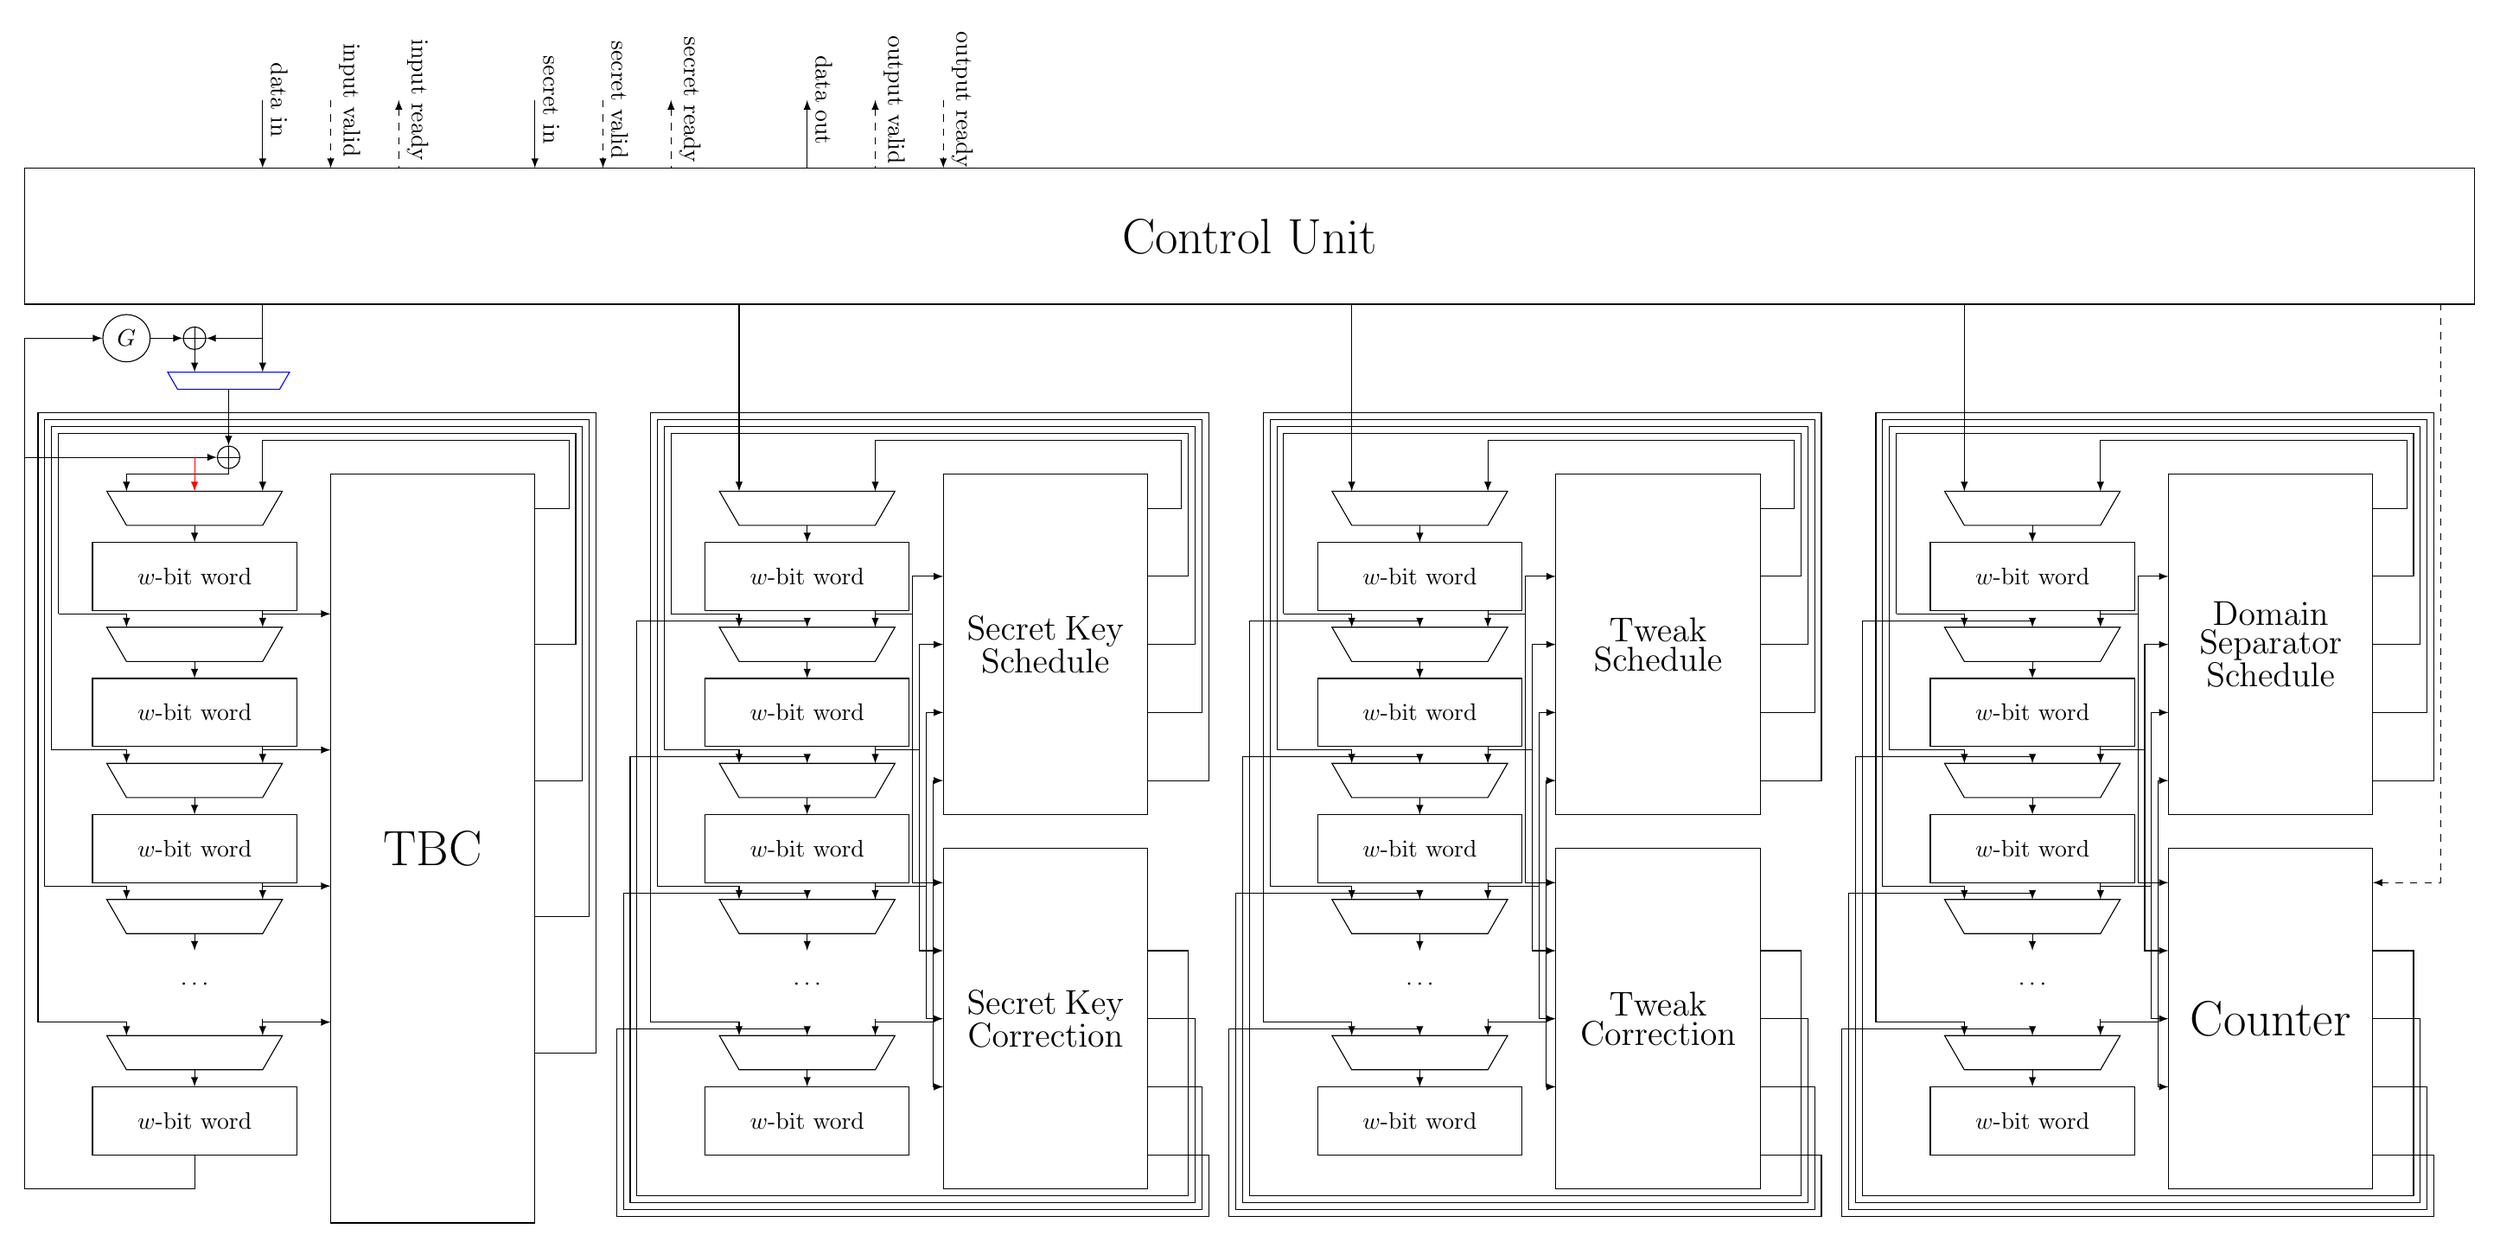
\begin{tikzpicture}
  \begin{scope}

    \node[draw,rectangle,minimum width=36cm,minimum height=2cm] (cu) at (15.5,5) {\huge  Control Unit};

    \draw[-latex] (1,7)node[above,rotate=-90]{data in}--(1,6) ;
    \draw[-latex,dashed] (2,7)node[above,rotate=-90]{input valid}--(2,6);
    \draw[latex-,dashed] (3,7)node[above,rotate=-90]{input ready}--(3,6);;

    \draw[-latex] (5,7)node[above,rotate=-90]{secret in}--(5,6);
    \draw[-latex,dashed] (6,7)node[above,rotate=-90]{secret valid}--(6,6);
    \draw[latex-,dashed] (7,7)node[above,rotate=-90]{secret ready}--(7,6);

    \draw[latex-] (9,7)node[above,rotate=-90]{data out}--(9,6);
    \draw[latex-,dashed] (10,7)node[above,rotate=-90]{output valid}--(10,6);
    \draw[-latex,dashed] (11,7)node[above,rotate=-90]{output ready}--(11,6);

  %\node[draw,circle,minimum width=1cm] (rho) at (-1,3) {$\rho$};

    \node[draw,circle,minimum width=0.5cm] (g) at (-1,3.5) {$G$};
    \node[draw,circle,minimum width=0.25cm] (x) at (0,3.5) {};
    \draw[-] (x.west)--(x.east);
    \draw[-] (x.north)--(x.south);

    \draw[-latex] (g.east)--(x.west);
    \draw[latex-] (x.east)--(1,3.5)--(1,4);
    \draw[-latex] (x.south)--(0,3);
    \draw[-latex] (1,3.5)--(1,3);
    \draw[color=blue] (-0.25,2.75)coordinate (O)--++(0:1.5)coordinate (A)--++(60:0.29)coordinate (B)--++(180:1.79)coordinate (C)--cycle;

    \node[draw,circle,minimum width=0.25cm] (x) at (0.5,1.75) {};
    \draw[-] (x.west)--(x.east);
    \draw[-] (x.north)--(x.south);
    \draw[-latex] (0.5,2.75)--(x.north);
    \draw[-latex] (x.south)--(0.5,1.5)--(-1,1.5)--(-1,1.25);

    \draw[-latex] (-2.5,1.75)--(x.west);
    \draw[-latex,color=red] (0,1.75)--(0,1.25);

  \node[draw,rectangle, minimum width=3cm, minimum height=1cm] (a) at (0,0){$w$-bit word};
  \node[draw,rectangle, minimum width=3cm, minimum height=1cm] (b) at (0,-2){$w$-bit word};
  \node[draw,rectangle, minimum width=3cm, minimum height=1cm] (c) at (0,-4){$w$-bit word};
  \node[minimum width=3cm, minimum height=1cm] (d) at (0,-6){$\cdots$};
  \node[draw,rectangle, minimum width=3cm, minimum height=1cm] (e) at (0,-8){$w$-bit word};

  \draw (-1,0.75)coordinate (O)--++(0:2)coordinate (A)--++(60:0.58)coordinate (B)--++(180:2.58)coordinate (C)--cycle;
  \draw[-latex] (0,0.75)--(0,0.5);

  \draw[-latex] (-2,-0.55)--(-1,-0.55)--(-1,-0.75);
  \draw[-latex] (1,-0.5)--(1,-0.75);
  \draw[-latex] (1,-0.55)--(2,-0.55);
  \draw (-1,-1.25)coordinate (O)--++(0:2)coordinate (A)--++(60:0.58)coordinate (B)--++(180:2.58)coordinate (C)--cycle;
  \draw[-latex] (0,-1.25)--(0,-1.5);

  \draw[-latex] (-2,-2.55)--(-1,-2.55)--(-1,-2.75);
  \draw[-latex] (1,-2.5)--(1,-2.75);
  \draw[-latex] (1,-2.55)--(2,-2.55);
  \draw (-1,-3.25)coordinate (O)--++(0:2)coordinate (A)--++(60:0.58)coordinate (B)--++(180:2.58)coordinate (C)--cycle;
  \draw[-latex] (0,-3.25)--(0,-3.5);

  \draw[-latex] (-2,-4.55)--(-1,-4.55)--(-1,-4.75);
  \draw[-latex] (1,-4.5)--(1,-4.75);
  \draw[-latex] (1,-4.55)--(2,-4.55);
  \draw (-1,-5.25)coordinate (O)--++(0:2)coordinate (A)--++(60:0.58)coordinate (B)--++(180:2.58)coordinate (C)--cycle;
  \draw[-latex] (0,-5.25)--(0,-5.5);

  \draw[-latex] (-2,-6.55)--(-1,-6.55)--(-1,-6.75);
  \draw[-latex] (1,-6.5)--(1,-6.75);
  \draw[-latex] (1,-6.55)--(2,-6.55);
  \draw (-1,-7.25)coordinate (O)--++(0:2)coordinate (A)--++(60:0.58)coordinate (B)--++(180:2.58)coordinate (C)--cycle;
  \draw[-latex] (0,-7.25)--(0,-7.5);

  \draw[-latex] (0,-8.5)--(0,-9)--(-2.5,-9)--(-2.5,3.5)--(g.west);

  \node[draw,rectangle,minimum width=3cm,minimum height=11cm] (tbc) at (3.5,-4) {\huge TBC};

  \draw[-latex] (5,1)--(5.5,1)--(5.5,2)--(1,2)--(1,1.25);
  \draw[-] (5,-1)--(5.6,-1)--(5.6,2.1)--(-2,2.1)--(-2,-0.55);
  \draw[-] (5,-3)--(5.7,-3)--(5.7,2.2)--(-2.1,2.2)--(-2.1,-2.55)--(-2,-2.55);
  \draw[-] (5,-5)--(5.8,-5)--(5.8,2.3)--(-2.2,2.3)--(-2.2,-4.55)--(-2,-4.55);
  \draw[-] (5,-7)--(5.9,-7)--(5.9,2.4)--(-2.3,2.4)--(-2.3,-6.55)--(-2,-6.55);
  \end{scope}

  \begin{scope}[xshift=9cm]

  \draw[latex-] (-1,1.25)--(-1,4);

  \node[draw,rectangle, minimum width=3cm, minimum height=1cm] (a) at (0,0){$w$-bit word};
  \node[draw,rectangle, minimum width=3cm, minimum height=1cm] (b) at (0,-2){$w$-bit word};
  \node[draw,rectangle, minimum width=3cm, minimum height=1cm] (c) at (0,-4){$w$-bit word};
  \node[minimum width=3cm, minimum height=1cm] (d) at (0,-6){$\cdots$};
  \node[draw,rectangle, minimum width=3cm, minimum height=1cm] (e) at (0,-8){$w$-bit word};


  \draw (-1,0.75)coordinate (O)--++(0:2)coordinate (A)--++(60:0.58)coordinate (B)--++(180:2.58)coordinate (C)--cycle;
  \draw[-latex] (0,0.75)--(0,0.5);

  \draw[-latex] (-2,-0.55)--(-1,-0.55)--(-1,-0.75);
  \draw[-latex] (-2.5,-0.65)--(0,-0.65)--(0,-0.75);
  \draw[-latex] (1,-0.5)--(1,-0.75);
  \draw[-latex] (1,-0.55)--(1.55,-0.55)--(1.55,0)--(2,0);
  \draw[-latex] (1.55,-0.55)--(1.55,-4.5)--(2,-4.5);
  \draw (-1,-1.25)coordinate (O)--++(0:2)coordinate (A)--++(60:0.58)coordinate (B)--++(180:2.58)coordinate (C)--cycle;
  \draw[-latex] (0,-1.25)--(0,-1.5);

  \draw[-latex] (-2,-2.55)--(-1,-2.55)--(-1,-2.75);
  \draw[-latex] (-2.5,-2.65)--(0,-2.65)--(0,-2.75);
  \draw[-latex] (1,-2.5)--(1,-2.75);
  \draw[-latex] (1,-2.55)--(1.65,-2.55)--(1.65,-1)--(2,-1);
  \draw[-latex] (1.65,-2.55)--(1.65,-5.5)--(2,-5.5);
  \draw (-1,-3.25)coordinate (O)--++(0:2)coordinate (A)--++(60:0.58)coordinate (B)--++(180:2.58)coordinate (C)--cycle;
  \draw[-latex] (0,-3.25)--(0,-3.5);

  \draw[-latex] (-2,-4.55)--(-1,-4.55)--(-1,-4.75);
  \draw[-latex] (-2.5,-4.65)--(0,-4.65)--(0,-4.75);
  \draw[-latex] (1,-4.5)--(1,-4.75);
  \draw[-latex] (1,-4.55)--(1.75,-4.55)--(1.75,-2)--(2,-2);
  \draw[-latex] (1.75,-4.55)--(1.75,-6.5)--(2,-6.5);
  \draw (-1,-5.25)coordinate (O)--++(0:2)coordinate (A)--++(60:0.58)coordinate (B)--++(180:2.58)coordinate (C)--cycle;
  \draw[-latex] (0,-5.25)--(0,-5.5);

  \draw[-latex] (-2,-6.55)--(-1,-6.55)--(-1,-6.75);
  \draw[-latex] (-2.5,-6.65)--(0,-6.65)--(0,-6.75);
  \draw[-latex] (1,-6.5)--(1,-6.75);
  \draw[-latex] (1,-6.55)--(1.85,-6.55)--(1.85,-3)--(2,-3);
  \draw[-latex] (1.85,-6.55)--(1.85,-7.5)--(2,-7.5);
  \draw (-1,-7.25)coordinate (O)--++(0:2)coordinate (A)--++(60:0.58)coordinate (B)--++(180:2.58)coordinate (C)--cycle;
  \draw[-latex] (0,-7.25)--(0,-7.5);

  \node[draw,rectangle,minimum width=3cm,minimum height=5cm,text width=2.5cm, align=center] (tbc) at (3.5,-1) {\Large Secret Key Schedule};

  \node[draw,rectangle,minimum width=3cm,minimum height=5cm,text width=2.5cm, align=center] (tbc) at (3.5,-6.5) {\Large Secret Key Correction};

  \draw[-latex] (5,1)--(5.5,1)--(5.5,2)--(1,2)--(1,1.25);
  \draw[-] (5,0)--(5.6,0)--(5.6,2.1)--(-2,2.1)--(-2,-0.55);
  \draw[-] (5,-1)--(5.7,-1)--(5.7,2.2)--(-2.1,2.2)--(-2.1,-2.55)--(-2,-2.55);
  \draw[-] (5,-2)--(5.8,-2)--(5.8,2.3)--(-2.2,2.3)--(-2.2,-4.55)--(-2,-4.55);
  \draw[-] (5,-3)--(5.9,-3)--(5.9,2.4)--(-2.3,2.4)--(-2.3,-6.55)--(-2,-6.55);

  \draw[-] (5,-5.5)--(5.6,-5.5)--(5.6,-9.1)--(-2.5,-9.1)--(-2.5,-0.65);
  \draw[-] (5,-6.5)--(5.7,-6.5)--(5.7,-9.2)--(-2.6,-9.2)--(-2.6,-2.65)--(-2.5,-2.65);
  \draw[-] (5,-7.5)--(5.8,-7.5)--(5.8,-9.3)--(-2.7,-9.3)--(-2.7,-4.65)--(-2.5,-4.65);
  \draw[-] (5,-8.5)--(5.9,-8.5)--(5.9,-9.4)--(-2.8,-9.4)--(-2.8,-6.65)--(-2.5,-6.65);
  \end{scope}

  \begin{scope}[xshift=18cm]

    \draw[latex-] (-1,1.25)--(-1,4);

  \node[draw,rectangle, minimum width=3cm, minimum height=1cm] (a) at (0,0){$w$-bit word};
  \node[draw,rectangle, minimum width=3cm, minimum height=1cm] (b) at (0,-2){$w$-bit word};
  \node[draw,rectangle, minimum width=3cm, minimum height=1cm] (c) at (0,-4){$w$-bit word};
  \node[minimum width=3cm, minimum height=1cm] (d) at (0,-6){$\cdots$};
  \node[draw,rectangle, minimum width=3cm, minimum height=1cm] (e) at (0,-8){$w$-bit word};


  \draw (-1,0.75)coordinate (O)--++(0:2)coordinate (A)--++(60:0.58)coordinate (B)--++(180:2.58)coordinate (C)--cycle;
  \draw[-latex] (0,0.75)--(0,0.5);

  \draw[-latex] (-2,-0.55)--(-1,-0.55)--(-1,-0.75);
  \draw[-latex] (-2.5,-0.65)--(0,-0.65)--(0,-0.75);
  \draw[-latex] (1,-0.5)--(1,-0.75);
  \draw[-latex] (1,-0.55)--(1.55,-0.55)--(1.55,0)--(2,0);
  \draw[-latex] (1.55,-0.55)--(1.55,-4.5)--(2,-4.5);
  \draw (-1,-1.25)coordinate (O)--++(0:2)coordinate (A)--++(60:0.58)coordinate (B)--++(180:2.58)coordinate (C)--cycle;
  \draw[-latex] (0,-1.25)--(0,-1.5);

  \draw[-latex] (-2,-2.55)--(-1,-2.55)--(-1,-2.75);
  \draw[-latex] (-2.5,-2.65)--(0,-2.65)--(0,-2.75);
  \draw[-latex] (1,-2.5)--(1,-2.75);
  \draw[-latex] (1,-2.55)--(1.65,-2.55)--(1.65,-1)--(2,-1);
  \draw[-latex] (1.65,-2.55)--(1.65,-5.5)--(2,-5.5);
  \draw (-1,-3.25)coordinate (O)--++(0:2)coordinate (A)--++(60:0.58)coordinate (B)--++(180:2.58)coordinate (C)--cycle;
  \draw[-latex] (0,-3.25)--(0,-3.5);

  \draw[-latex] (-2,-4.55)--(-1,-4.55)--(-1,-4.75);
  \draw[-latex] (-2.5,-4.65)--(0,-4.65)--(0,-4.75);
  \draw[-latex] (1,-4.5)--(1,-4.75);
  \draw[-latex] (1,-4.55)--(1.75,-4.55)--(1.75,-2)--(2,-2);
  \draw[-latex] (1.75,-4.55)--(1.75,-6.5)--(2,-6.5);
  \draw (-1,-5.25)coordinate (O)--++(0:2)coordinate (A)--++(60:0.58)coordinate (B)--++(180:2.58)coordinate (C)--cycle;
  \draw[-latex] (0,-5.25)--(0,-5.5);

  \draw[-latex] (-2,-6.55)--(-1,-6.55)--(-1,-6.75);
  \draw[-latex] (-2.5,-6.65)--(0,-6.65)--(0,-6.75);
  \draw[-latex] (1,-6.5)--(1,-6.75);
  \draw[-latex] (1,-6.55)--(1.85,-6.55)--(1.85,-3)--(2,-3);
  \draw[-latex] (1.85,-6.55)--(1.85,-7.5)--(2,-7.5);
  \draw (-1,-7.25)coordinate (O)--++(0:2)coordinate (A)--++(60:0.58)coordinate (B)--++(180:2.58)coordinate (C)--cycle;
  \draw[-latex] (0,-7.25)--(0,-7.5);

  \node[draw,rectangle,minimum width=3cm,minimum height=5cm,text width=2.5cm, align=center] (tbc) at (3.5,-1) {\Large Tweak Schedule};

  \node[draw,rectangle,minimum width=3cm,minimum height=5cm,text width=2.5cm, align=center] (tbc) at (3.5,-6.5) {\Large Tweak Correction};

  \draw[-latex] (5,1)--(5.5,1)--(5.5,2)--(1,2)--(1,1.25);
  \draw[-] (5,0)--(5.6,0)--(5.6,2.1)--(-2,2.1)--(-2,-0.55);
  \draw[-] (5,-1)--(5.7,-1)--(5.7,2.2)--(-2.1,2.2)--(-2.1,-2.55)--(-2,-2.55);
  \draw[-] (5,-2)--(5.8,-2)--(5.8,2.3)--(-2.2,2.3)--(-2.2,-4.55)--(-2,-4.55);
  \draw[-] (5,-3)--(5.9,-3)--(5.9,2.4)--(-2.3,2.4)--(-2.3,-6.55)--(-2,-6.55);

  \draw[-] (5,-5.5)--(5.6,-5.5)--(5.6,-9.1)--(-2.5,-9.1)--(-2.5,-0.65);
  \draw[-] (5,-6.5)--(5.7,-6.5)--(5.7,-9.2)--(-2.6,-9.2)--(-2.6,-2.65)--(-2.5,-2.65);
  \draw[-] (5,-7.5)--(5.8,-7.5)--(5.8,-9.3)--(-2.7,-9.3)--(-2.7,-4.65)--(-2.5,-4.65);
  \draw[-] (5,-8.5)--(5.9,-8.5)--(5.9,-9.4)--(-2.8,-9.4)--(-2.8,-6.65)--(-2.5,-6.65);
  \end{scope}

  \begin{scope}[xshift=27cm]

    \draw[latex-,dashed] (5,-4.5)--(6,-4.5)--(6,4);

  \draw[latex-] (-1,1.25)--(-1,4);

  \node[draw,rectangle, minimum width=3cm, minimum height=1cm] (a) at (0,0){$w$-bit word};
  \node[draw,rectangle, minimum width=3cm, minimum height=1cm] (b) at (0,-2){$w$-bit word};
  \node[draw,rectangle, minimum width=3cm, minimum height=1cm] (c) at (0,-4){$w$-bit word};
  \node[minimum width=3cm, minimum height=1cm] (d) at (0,-6){$\cdots$};
  \node[draw,rectangle, minimum width=3cm, minimum height=1cm] (e) at (0,-8){$w$-bit word};


  \draw (-1,0.75)coordinate (O)--++(0:2)coordinate (A)--++(60:0.58)coordinate (B)--++(180:2.58)coordinate (C)--cycle;
  \draw[-latex] (0,0.75)--(0,0.5);

  \draw[-latex] (-2,-0.55)--(-1,-0.55)--(-1,-0.75);
  \draw[-latex] (-2.5,-0.65)--(0,-0.65)--(0,-0.75);
  \draw[-latex] (1,-0.5)--(1,-0.75);
  \draw[-latex] (1,-0.55)--(1.55,-0.55)--(1.55,0)--(2,0);
  \draw[-latex] (1.55,-0.55)--(1.55,-4.5)--(2,-4.5);
  \draw (-1,-1.25)coordinate (O)--++(0:2)coordinate (A)--++(60:0.58)coordinate (B)--++(180:2.58)coordinate (C)--cycle;
  \draw[-latex] (0,-1.25)--(0,-1.5);

  \draw[-latex] (-2,-2.55)--(-1,-2.55)--(-1,-2.75);
  \draw[-latex] (-2.5,-2.65)--(0,-2.65)--(0,-2.75);
  \draw[-latex] (1,-2.5)--(1,-2.75);
  \draw[-latex] (1,-2.55)--(1.65,-2.55)--(1.65,-1)--(2,-1);
  \draw[-latex] (1.65,-2.55)--(1.65,-5.5)--(2,-5.5);
  \draw (-1,-3.25)coordinate (O)--++(0:2)coordinate (A)--++(60:0.58)coordinate (B)--++(180:2.58)coordinate (C)--cycle;
  \draw[-latex] (0,-3.25)--(0,-3.5);

  \draw[-latex] (-2,-4.55)--(-1,-4.55)--(-1,-4.75);
  \draw[-latex] (-2.5,-4.65)--(0,-4.65)--(0,-4.75);
  \draw[-latex] (1,-4.5)--(1,-4.75);
  \draw[-latex] (1,-4.55)--(1.75,-4.55)--(1.75,-2)--(2,-2);
  \draw[-latex] (1.75,-4.55)--(1.75,-6.5)--(2,-6.5);
  \draw (-1,-5.25)coordinate (O)--++(0:2)coordinate (A)--++(60:0.58)coordinate (B)--++(180:2.58)coordinate (C)--cycle;
  \draw[-latex] (0,-5.25)--(0,-5.5);

  \draw[-latex] (-2,-6.55)--(-1,-6.55)--(-1,-6.75);
  \draw[-latex] (-2.5,-6.65)--(0,-6.65)--(0,-6.75);
  \draw[-latex] (1,-6.5)--(1,-6.75);
  \draw[-latex] (1,-6.55)--(1.85,-6.55)--(1.85,-3)--(2,-3);
  \draw[-latex] (1.85,-6.55)--(1.85,-7.5)--(2,-7.5);
  \draw (-1,-7.25)coordinate (O)--++(0:2)coordinate (A)--++(60:0.58)coordinate (B)--++(180:2.58)coordinate (C)--cycle;
  \draw[-latex] (0,-7.25)--(0,-7.5);

  \node[draw,rectangle,minimum width=3cm,minimum height=5cm,text width=2.5cm, align=center] (tbc) at (3.5,-1) {\Large Domain Separator Schedule};

  \node[draw,rectangle,minimum width=3cm,minimum height=5cm,text width=2.5cm, align=center] (tbc) at (3.5,-6.5) {\huge Counter};

  \draw[-latex] (5,1)--(5.5,1)--(5.5,2)--(1,2)--(1,1.25);
  \draw[-] (5,0)--(5.6,0)--(5.6,2.1)--(-2,2.1)--(-2,-0.55);
  \draw[-] (5,-1)--(5.7,-1)--(5.7,2.2)--(-2.1,2.2)--(-2.1,-2.55)--(-2,-2.55);
  \draw[-] (5,-2)--(5.8,-2)--(5.8,2.3)--(-2.2,2.3)--(-2.2,-4.55)--(-2,-4.55);
  \draw[-] (5,-3)--(5.9,-3)--(5.9,2.4)--(-2.3,2.4)--(-2.3,-6.55)--(-2,-6.55);

  \draw[-] (5,-5.5)--(5.6,-5.5)--(5.6,-9.1)--(-2.5,-9.1)--(-2.5,-0.65);
  \draw[-] (5,-6.5)--(5.7,-6.5)--(5.7,-9.2)--(-2.6,-9.2)--(-2.6,-2.65)--(-2.5,-2.65);
  \draw[-] (5,-7.5)--(5.8,-7.5)--(5.8,-9.3)--(-2.7,-9.3)--(-2.7,-4.65)--(-2.5,-4.65);
  \draw[-] (5,-8.5)--(5.9,-8.5)--(5.9,-9.4)--(-2.8,-9.4)--(-2.8,-6.65)--(-2.5,-6.65);
  \end{scope}
\end{tikzpicture}


\end{document}
